\section{Graphics Pipeline}

The graphics pipeline gained popularity thanks to the OpenGL API for graphics
that released in 1989. It's popularity inspired hardware to dedicate individual units
to its tasks, leading to many graphics accelerators implementing this pipeline in hardware
\cite{mcclanahan2010history}.

The pipeline covered here has four primary stages (\cite{crow2004evolution}):

\begin{itemize}
    \item Application
    \item Geometry
    \item Rasterization
    \item Screen
\end{itemize}

with other minor stages scattered between.

This section will explain these stages and use them to narrate the evolution of the unprogrammable graphics accelerators commonplace in the 1980s into the general purpose hardware we are familiar with.
More details can be found in the references, as well as in the Wikipedia page for
the Graphics Pipeline which covers the same sections as this report \cite{wiki:Graphics_pipeline}.

\subsection{Application}

We can understand the \textit{Application} stage by starting from its output.
Its output includes a set of vertices that encode information pertaining to objects to be rendered onto the screen and their transformations.
The \textit{Application} stage, then, naturally does the tasks necessary to produce or update the information encoded in these vertices.
These tasks vary based on the application, but examples include handling physics in video games and animation.

The information encoded in vertices varies based on implementation. OpenGL's vertices include position, normal, and color (\cite{wiki:vertex}).

\subsection{Geometry}

The next stage of the pipeline is the \textit{Geometry} stage. 
This consists of a number of substages.

\textbf{Transformation:}
Vertices represent objects but are unlikely to be in the correct position in space.
These vertices are first transformed to where they should be in space.
For a concrete example: if a programmer specifies a car's coordinates and
rotation, the first part of the \textit{Transformation} stage would be to perform
transformations (typically via matrix multiplication) to get the car in the
right place [\cite{nvidia256}].

In addition to objects, an observer exists somewhere in space.
The observer has a set of coordinates, a rotation, and a field of view that altogether dictate the view that should get rendered to the screen.
In hardware, however, the observer's parameters are fixed with its position at the origin.
Thus, we must transform our space to have the observer at this position.
With this transformation, what the observer sees does not change.
In this transformation, the 2D plane corresponding to what the observer
sees is typically mapped to the $x,y$ directions and the depth to $z$.
Perspective transformations are also applied here to make what the observer sees in the $x,y$ plane correspond to our perception of 3D space \cite{agoston2005transformations}.

\begin{figure}[h]
    \centering
    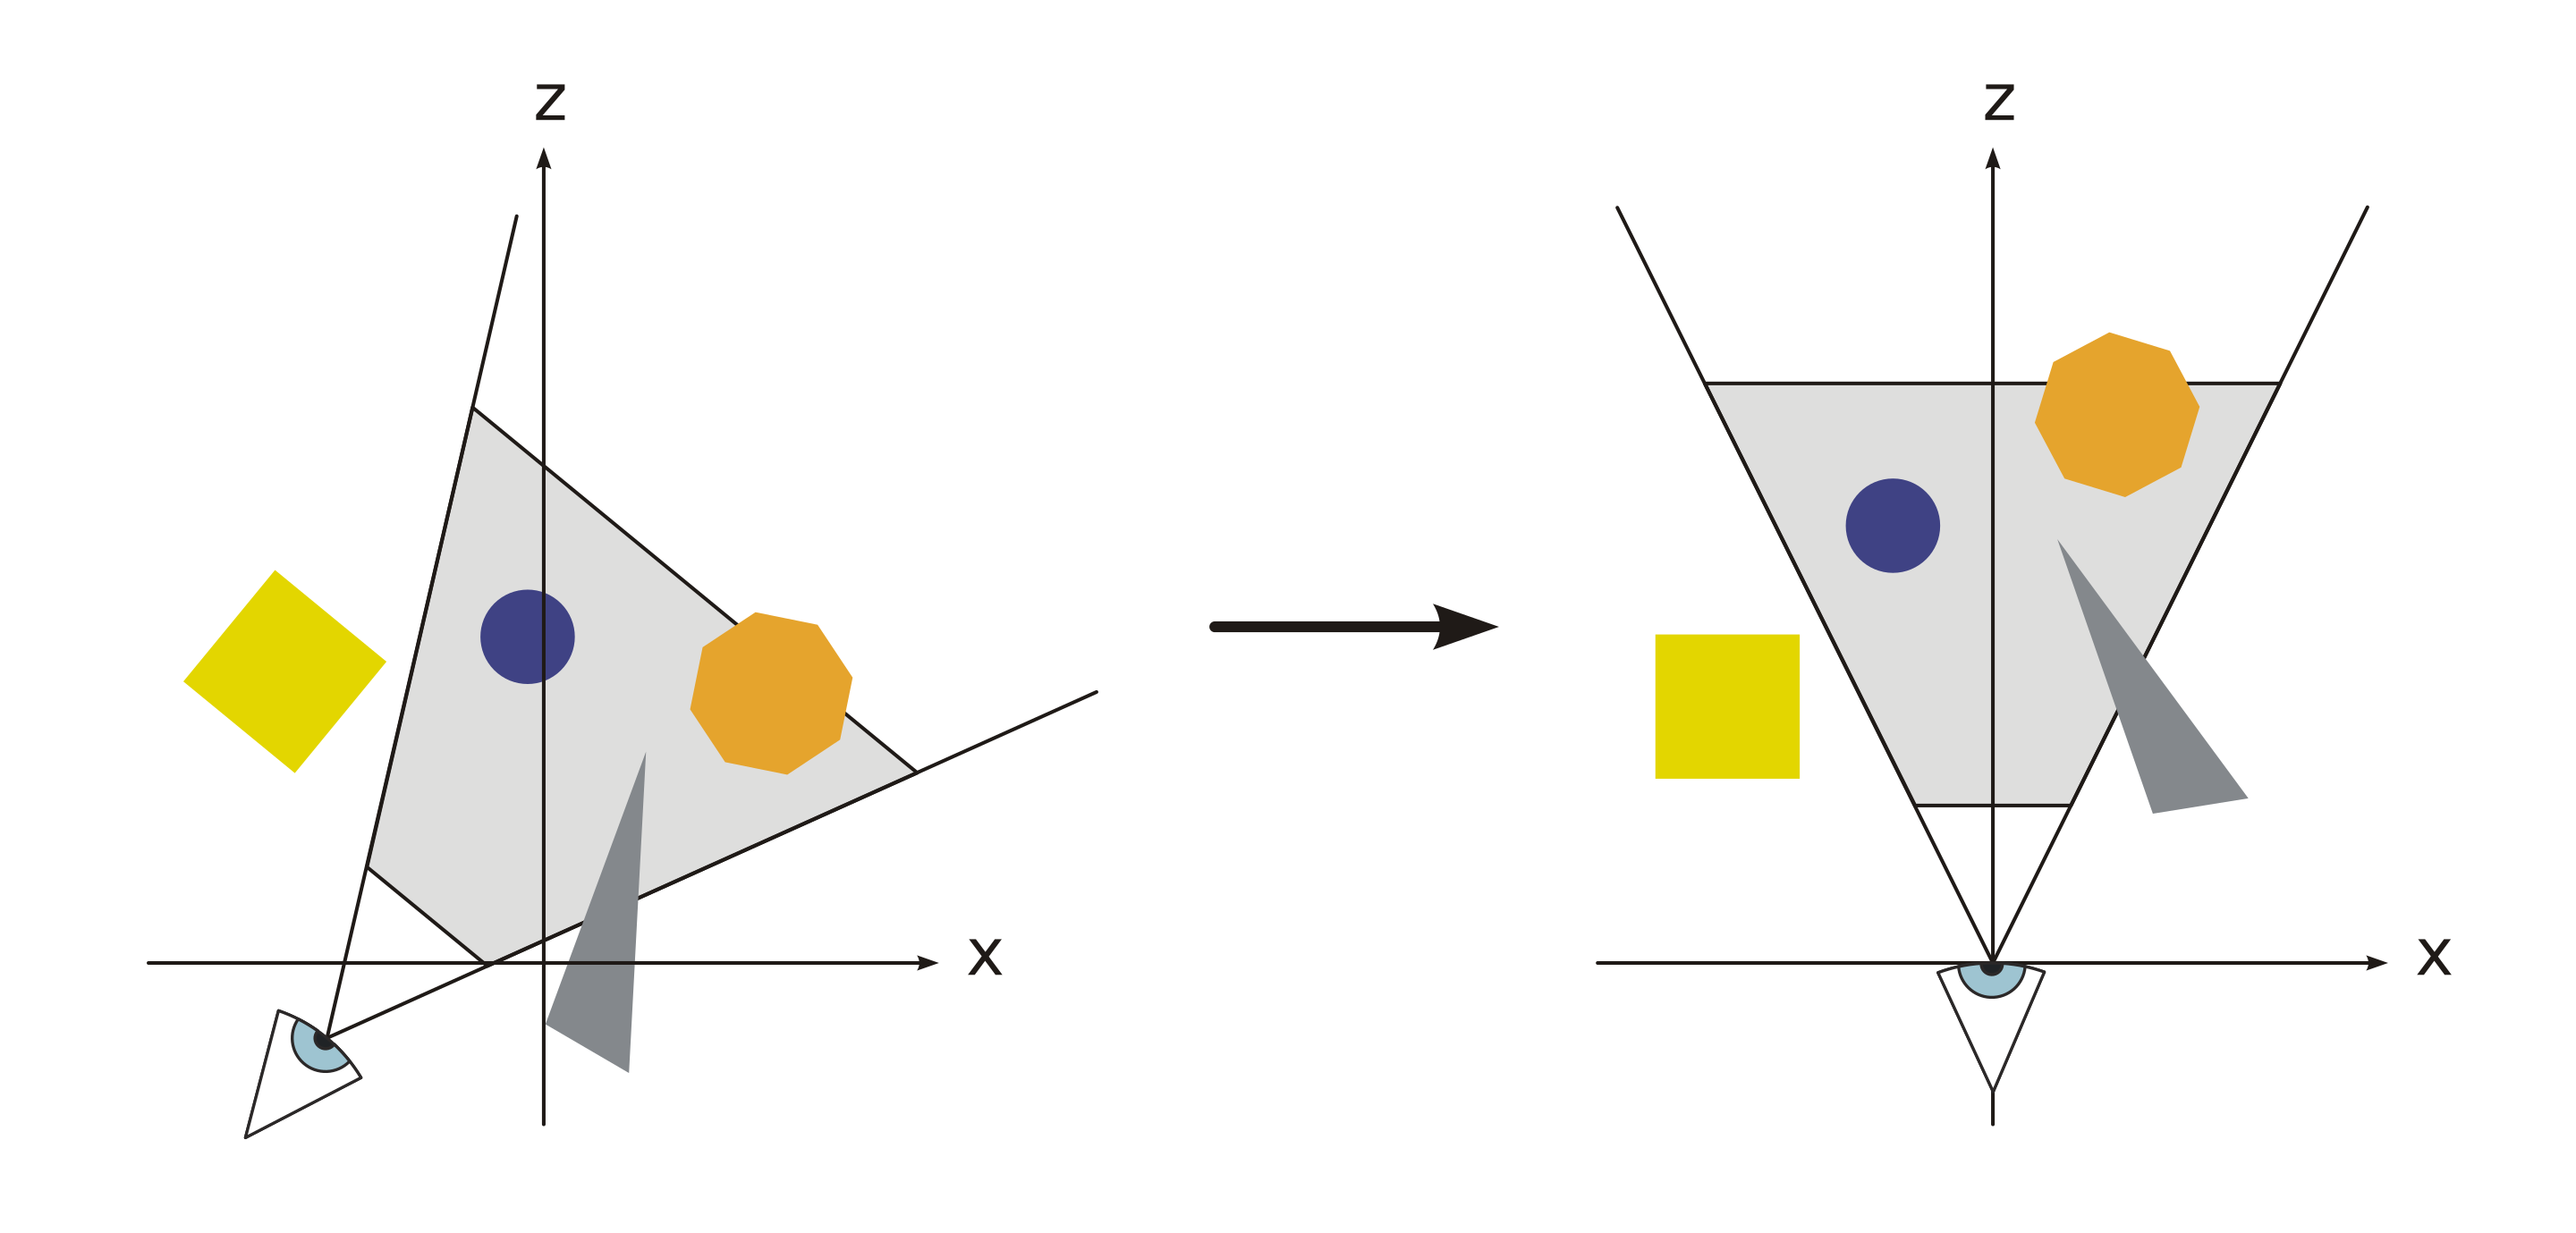
\includegraphics[width=0.5\textwidth]{assets/View_transform.png}
    \caption{Transformation of the space to fit the observer.}
    \label{fig:transform}
\end{figure}

An example of this can be seen in Figure \ref{fig:transform} taken from \cite{wiki:Graphics_pipeline}.

\textbf{Lighting:}
The \textit{Lighting} stage modifies the color values of our transformed vertices.
Lighting information is given to us by the \textit{Application} stage.
This includes information about light sources, like spot lights and ambient
light, including their strength and orientation.
This information is largely encoded in matrices and the color values of
vertices can be modified with a series of matrix multiplications[\cite{nvidia256}].

\textbf{Primitive Assembly:}
This stage groups our vertices into triangles and other primitives.
Triangles are the simplest polygon that we can combine to create other polygons,
making them convenient to work with (\cite{wiki:overview}, \cite{scratchapixelRasterization}).

\textbf{Clipping and Culling:}
The world our space represents may have objects that the observer can't see.
The primitives composing these objects are entirely removed in what is called \textbf{culling} \cite{graphicscompendiumGraphicsCompendium}.

Some objects overlap with the boundaries of the observer's field of view. The
triangles making up these objects are reshaped --- converted into smaller traingles ---
to fit within the boundaries.
This process is called \textbf{clipping} \cite{graphicscompendiumGraphicsCompendium}.

An example of clipping and culling can be found in Figure \ref{fig:clip} taken from \cite{wiki:Graphics_pipeline}.

\begin{figure}[h]
    \centering
    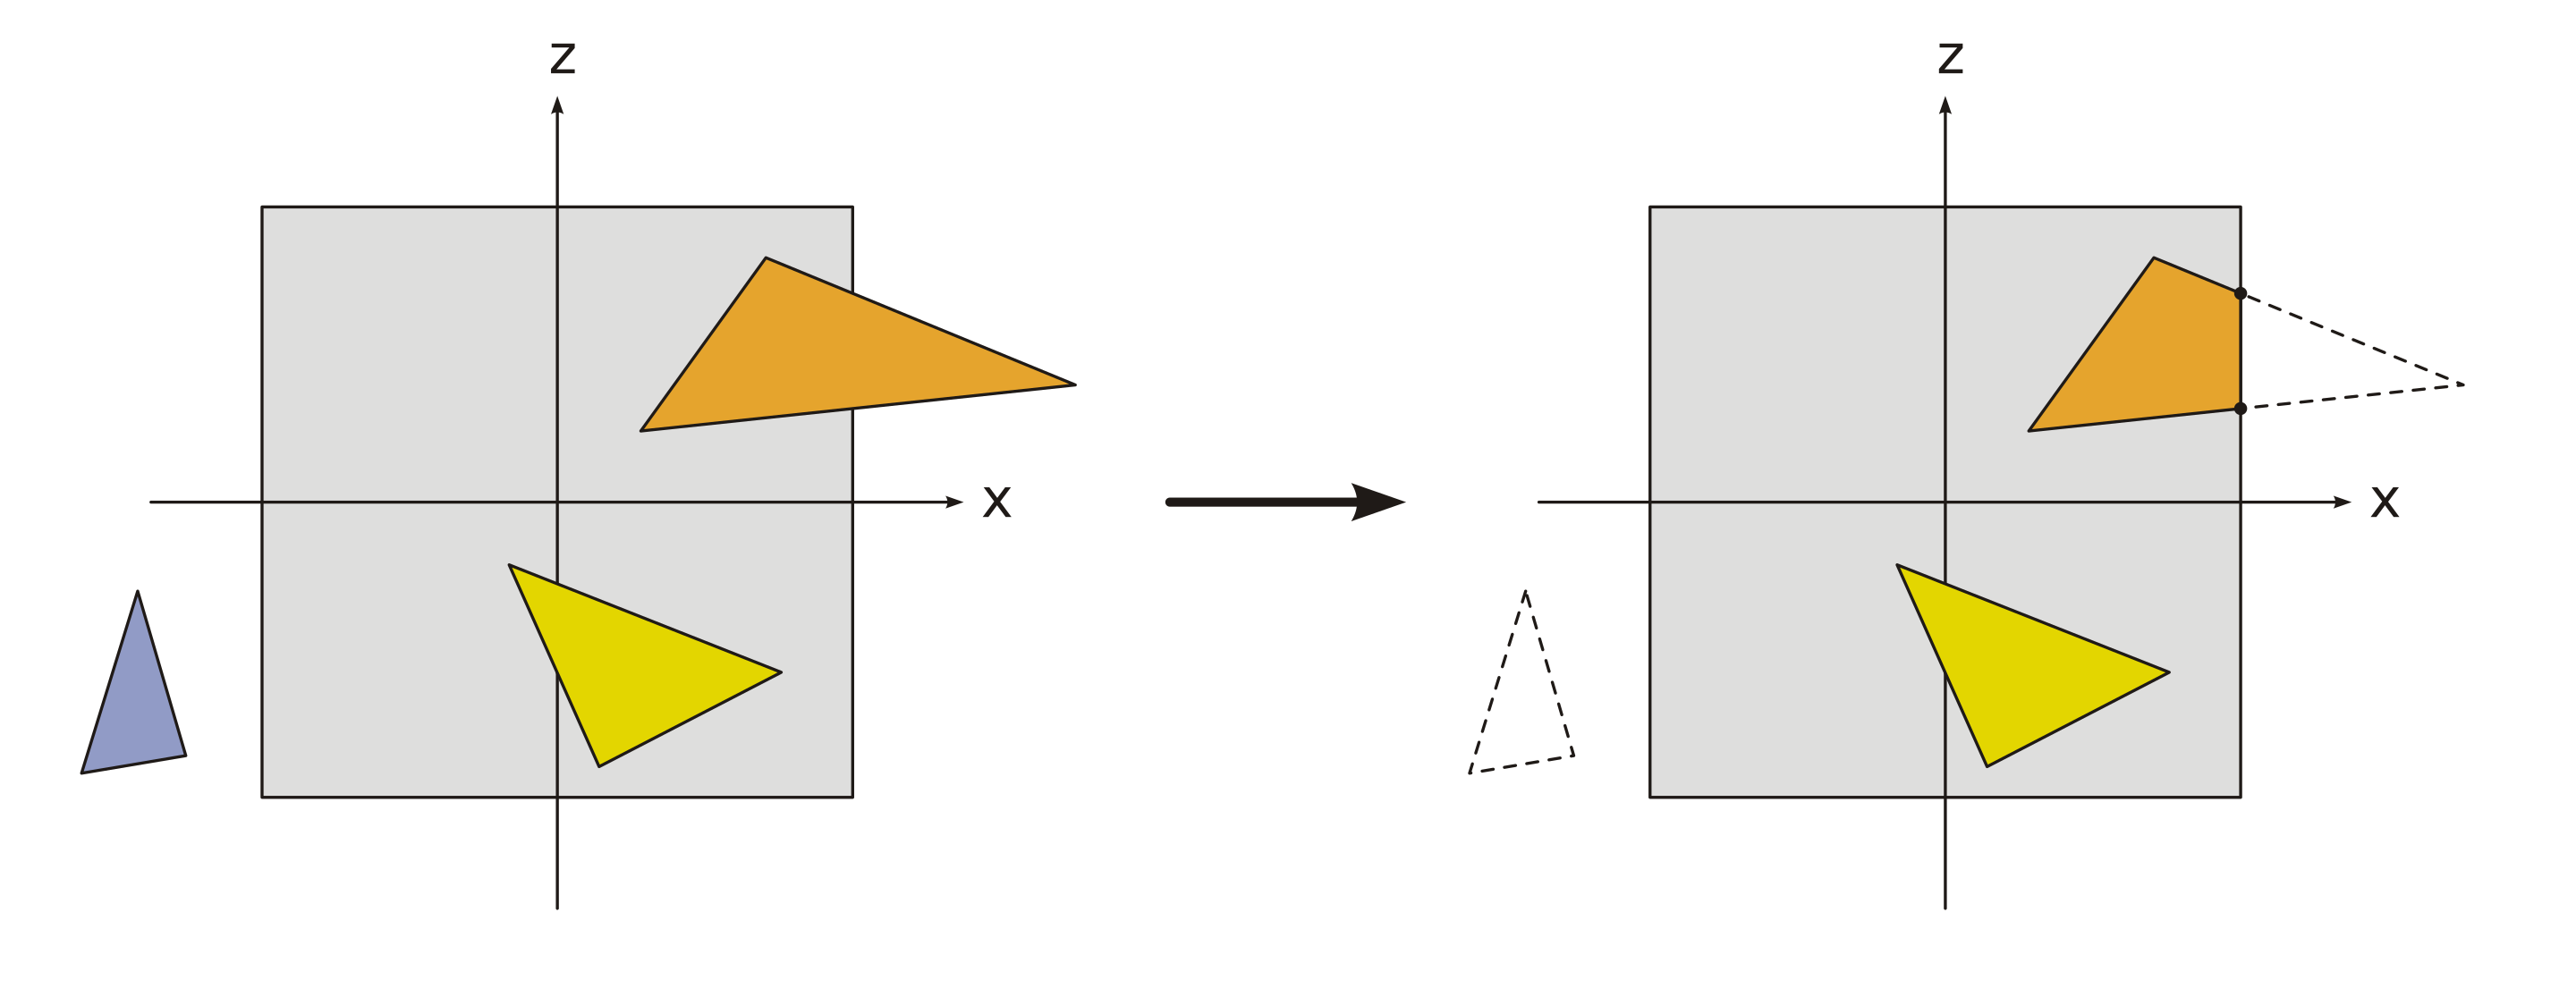
\includegraphics[width=0.5\textwidth]{assets/Cube_clipping.png}
    \caption{Examples of clipping (of the blue triangle) and culling (of the orange triangle). }
    \label{fig:clip}
\end{figure}

\subsection{Rasterization}

After we pass the \textit{Geometry} stage, we have a set of triangles.
This stage converts those triangles into fragments.

Fragments can be generated through the following algorithm:
First, iterate through all triangles. Next, iterate over all pixels.
If a triangle overlaps with a pixel, create a fragment with those pixel
coordinates belonging to the triangle \cite{scratchapixelRasterization}.

Fragments differ from pixels in that there can be multiple fragments corresponding
to a given pixel's position on the screen. In terms of storing color information,
they are the same.

Fragments are used in later minor stages of the pipeline.

\subsection{Screen}
The pipeline ends with fragments rendered to the screen as pixels.
Rendering happens through writing colour data to a special region in memory
mapped to the screen.
